\documentclass[xcolor=dvipsnames]{beamer}

\setbeamertemplate{navigation symbols}{}
%\setbeamertemplate{background}[grid][step=1cm]
\useoutertheme{infolines}
\usepackage{graphicx}
\usepackage{xspace}
\usepackage{hyperref}

\hypersetup{
  pdftitle={Status of Field Calculations}
  pdfauthor={Brett Viren},
  colorlinks=true,
  linkcolor=DarkOrchid,
  urlcolor=DarkOrchid,
}

\newcommand{\microboone}{MicroBooNE\xspace}

\date{\today}

\begin{document}

\begin{frame}{Status of Field Calculations}
  \tableofcontents
\end{frame}

\section{Methods}

\begin{frame}[fragile]
  \frametitle{Weighting Potential}
  \href{https://en.wikipedia.org/wiki/Shockley%E2%80%93Ramo_theorem}{Shockley-Ramo} construction:
  \begin{enumerate}
  \item Identify one electrode, $k$.
  \item Set to unit voltage, all others set to 0V.
  \item Calculate its \textit{weighting} potential $\phi_{weight,k}$ in the volume.
  \item Calculate the associated E-field $\vec{E}_{weight,k}$.
  \item Calculate the overall \textit{drift} potential and E-field
    $\vec{E}_{drift}$.
  \end{enumerate}
  Induced current on the electrode $k$ from charge $q$ moving with velocity $\vec{v}$:
  \begin{center}
    $i_k = q \vec{E}_{weight,k} \cdot \vec{v}$
  \end{center}
  And, electron drift velocity, for given mobility $\mu$:
  \begin{center}
    $\vec{v} = \mu \vec{E}_{drift}$
  \end{center}

\end{frame}

\begin{frame}
  \frametitle{Boundary Element Method for Electrostatic Potential}

  \begin{enumerate}
  \item Discretize (mesh) boundary electrodes.
  \item Define potential on each mesh element.
  \item Integrate Laplace $\nabla^2\phi=0$.
  \item Fit integral equations to boundary values.
  \item Evaluate solution on points in the volume.
  \end{enumerate}

\end{frame}

\begin{frame}
  \frametitle{Element Methods: Boundary vs. Finite}
  \begin{columns}
    \begin{column}{0.5\textwidth}
      BEM
      \begin{itemize}
      \item Meshes the surfaces.
      \item Fast for low surface-to-volume.
      \item Performance relies on relatively new math discoveries.
      \item Relatively few software implementations.
      \end{itemize}      
    \end{column}
    \begin{column}{0.5\textwidth}
      FEM
      \begin{itemize}
      \item Meshes the volume.
      \item Fast for high surface-to-volume.
      \item Adaptive meshes can improve performance.
      \item Many implementations, heavily used in industry.
      \end{itemize}      
    \end{column}
  \end{columns}
\end{frame}

\section{Geometries}

\begin{frame}{Status of Field Calculations}
  \tableofcontents[currentsection]
\end{frame}

\begin{frame}{Wires Meshes}

  \footnotesize

  \begin{columns}
    \begin{column}{0.3\textwidth}
      \begin{center}
        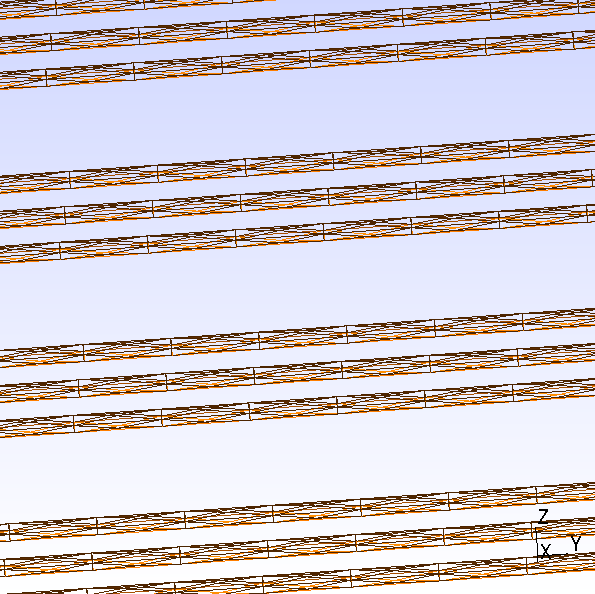
\includegraphics[height=0.4\textheight]{parallel-mesh.png}      
        
        ``Parallel'':\\3mm pitch and gap\\all wires parallel
      \end{center}
    \end{column}
    \begin{column}{0.3\textwidth}
      \begin{center}
        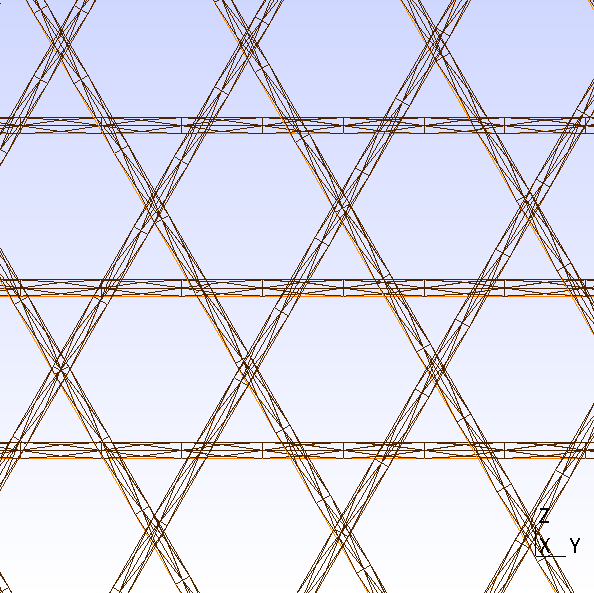
\includegraphics[height=0.4\textheight]{uboone-mesh.png}      

        ``\microboone'':\\3mm pitch and gap\\$60^\circ$ angles for U/V.
      \end{center}
    \end{column}
    \begin{column}{0.3\textwidth}
      \begin{center}
        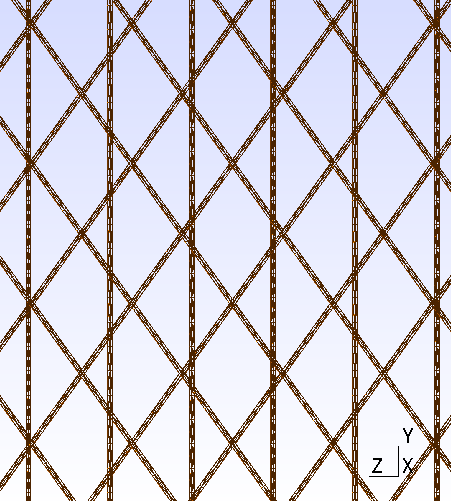
\includegraphics[height=0.4\textheight]{dune-mesh.png}      

        ``DUNE'':\\5mm pitch and gap\\$35.7^\circ$ angles for U/V.
      \end{center}
    \end{column}
  \end{columns}
\end{frame}


\begin{frame}{Add Cathode (\microboone)}
  \begin{center}
    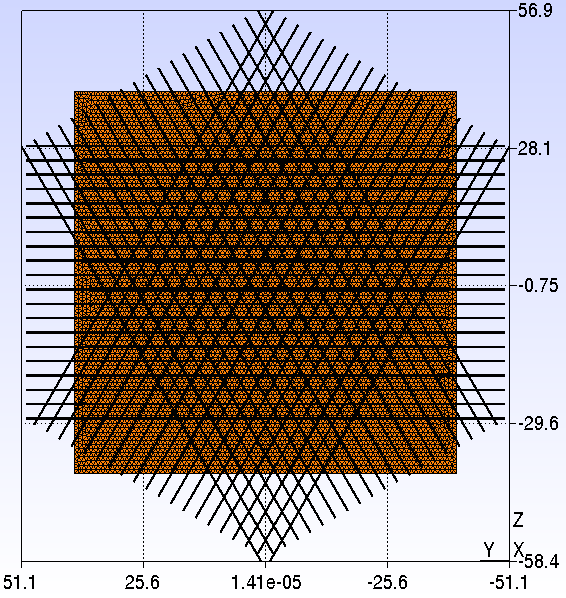
\includegraphics[height=0.7\textheight]{uboone-mesh-with-plate.png}%
    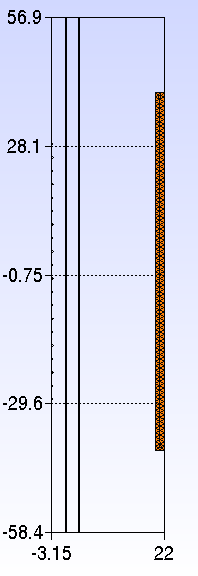
\includegraphics[height=0.7\textheight]{uboone-mesh-with-plate-side.png}      

    \begin{itemize}
    \item ``Cathode'' is near wires with voltage adjusted to give 500V/cm.
    \item Do calculations at center, far enough away from edge effects.
    \end{itemize}
  \end{center}
\end{frame}

\section{Weighting Potentials}

\begin{frame}{Status of Field Calculations}
  \tableofcontents[currentsection]
\end{frame}

\begin{frame}
  \frametitle{Weighting Potential - 2D vs ``2D''}

  \vspace{-5mm}

  \begin{columns}
    \begin{column}{0.5\textwidth}
      \begin{center}
        \includegraphics[height=0.65\textheight,page=5,angle=-90,clip,trim=0 0 0 5mm]{GarfieldSimulation-BoYu.pdf}

        \scriptsize Garfield 2D calculation from Bo
      \end{center}
    \end{column}
    \begin{column}{0.5\textwidth}
      \begin{center}
        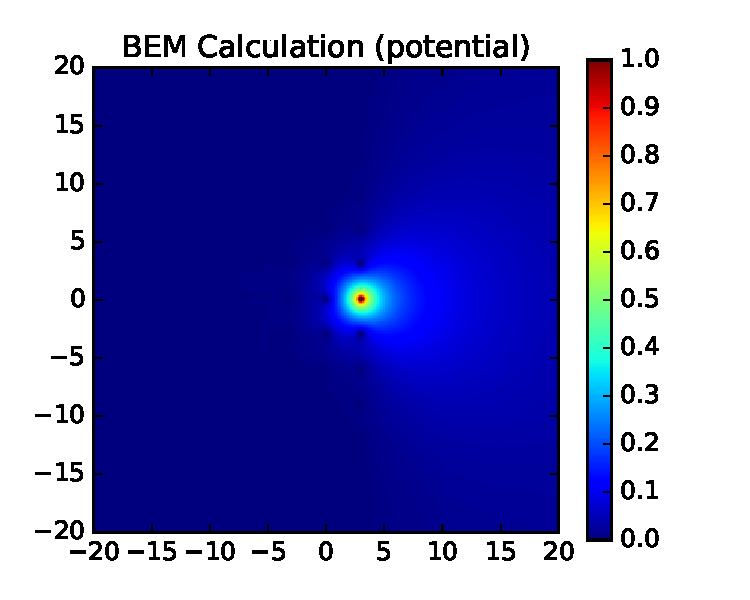
\includegraphics[height=0.65\textheight]{parallel-near-d11.pdf}

        \scriptsize 3D BEM, parallel wires, sliced at Y=0.
      \end{center}
    \end{column}
  \end{columns}

  \begin{center}
    Initial, qualitative agreement.  More checks needed.
  \end{center}

\end{frame}

\begin{frame}{Weighting Potential - 2D vs. 3D wire pattern}

  \vspace{-5mm}

  \begin{columns}
    \begin{column}{0.5\textwidth}
      \begin{center}
        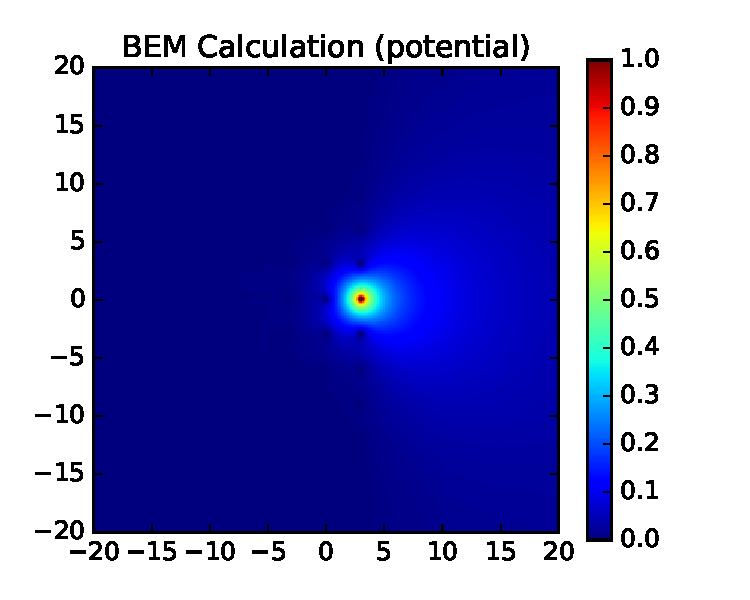
\includegraphics[height=0.65\textheight]{parallel-near-d11.pdf}

        \scriptsize Parallel wires
      \end{center}
    \end{column}
    \begin{column}{0.5\textwidth}
      \begin{center}
        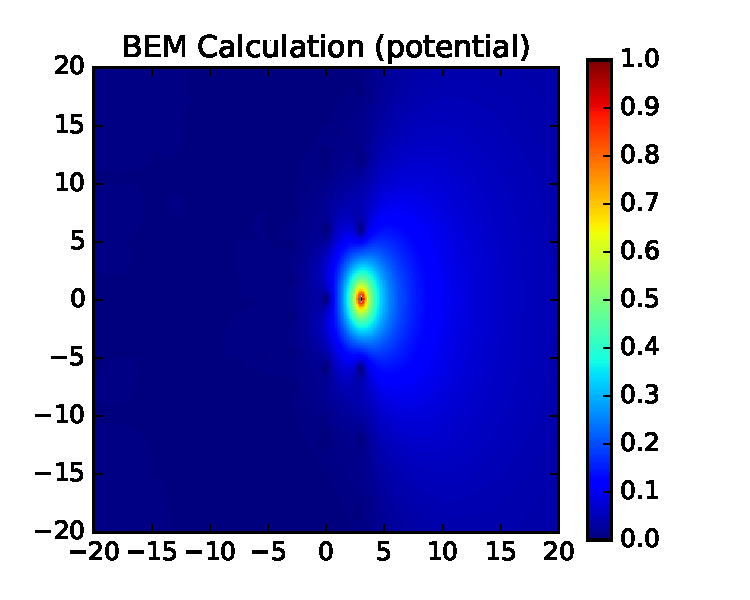
\includegraphics[height=0.65\textheight]{uboone-near-d11.pdf}

        \scriptsize \microboone wires.
      \end{center}
    \end{column}
  \end{columns}

  \begin{center}
    Clear distortion in extent and shape.  Not surprising.
  \end{center}

\end{frame}

\section{Drift Potentials and Fields}

\begin{frame}{Status of Field Calculations}
  \tableofcontents[currentsection]
\end{frame}

\begin{frame}{Capacitor}
  \begin{center}
    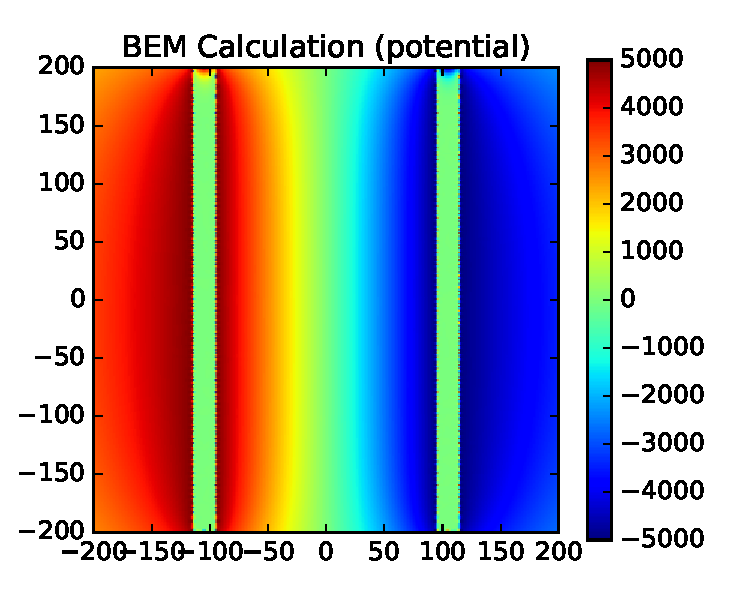
\includegraphics[height=0.8\textheight]{capacitor-drift-full.pdf}

    Simple test with parallel-plates at +/-5000V.

  \end{center}
\end{frame}

\begin{frame}{Drift Potential - 2D vs. 3D wire pattern}

  \begin{columns}
    \begin{column}{0.5\textwidth}
      \begin{center}
        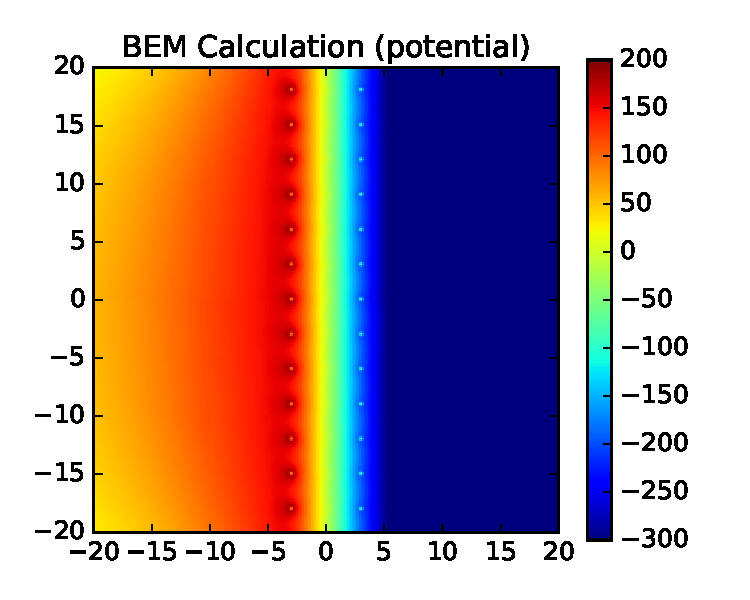
\includegraphics[height=0.6\textheight]{wirescpa-drift-near.pdf}

        \scriptsize Parallel wires
      \end{center}
    \end{column}
    \begin{column}{0.5\textwidth}
      \begin{center}
        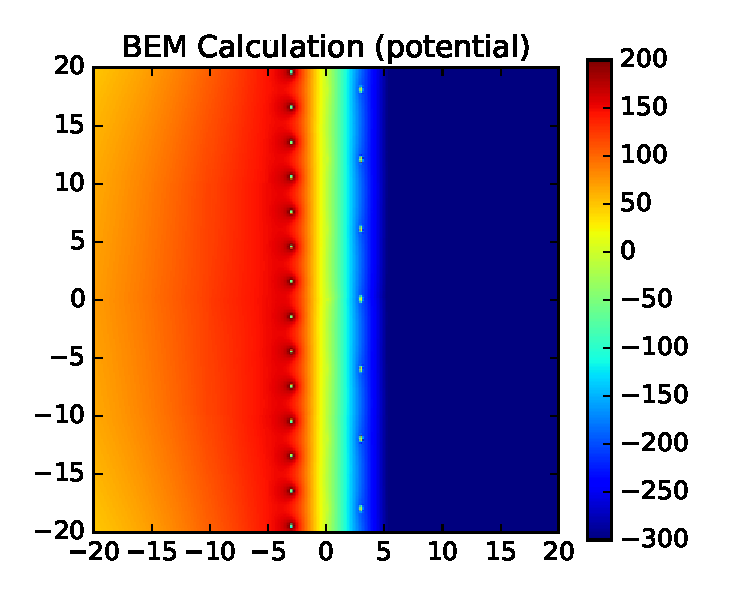
\includegraphics[height=0.6\textheight]{uboone-drift-near.pdf}

        \scriptsize \microboone wires.
      \end{center}
    \end{column}
  \end{columns}
  \begin{center}
    Electrodes (from left-to-right) W $\rightarrow$ V  $\rightarrow$ U  $\rightarrow$ Cathode (off scale)
  \end{center}

\end{frame}

\begin{frame}
  \frametitle{Some Issues - Mesh Granularity}

  \vspace{-5mm}

  \begin{columns}
    \begin{column}{0.5\textwidth}
      \begin{center}
        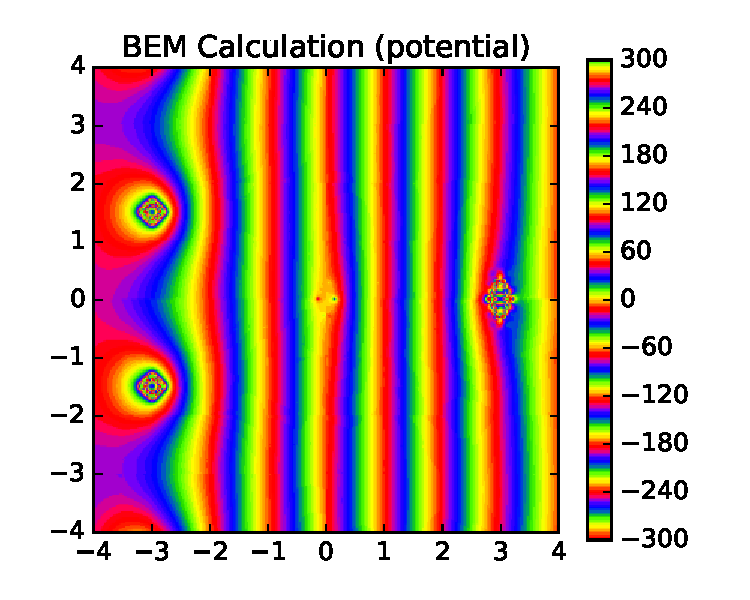
\includegraphics[height=0.6\textheight]{fluctuations1.pdf}

        \scriptsize Major features look okay.
      \end{center}
    \end{column}
    \begin{column}{0.5\textwidth}
      \begin{center}
        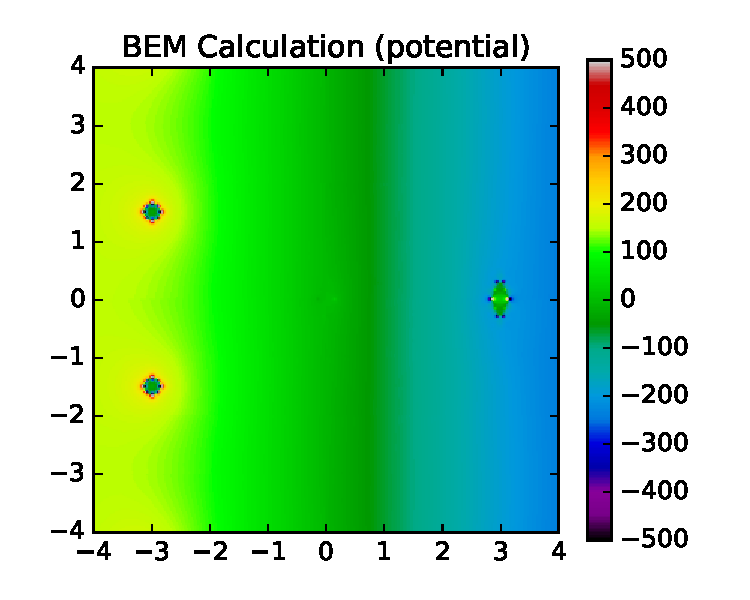
\includegraphics[height=0.6\textheight]{fluctuations2.pdf}

        \scriptsize Large +/- fluctuations near wires.
      \end{center}
    \end{column}
  \end{columns}
  
  \vfill
  \begin{itemize}
  \item Drift potential has large fluctuations right near the wires.
  \end{itemize}
\end{frame}

\begin{frame}
  \frametitle{Wire Mesh Closeup}
  \begin{columns}
    \begin{column}{0.5\textwidth}
      \begin{center}
        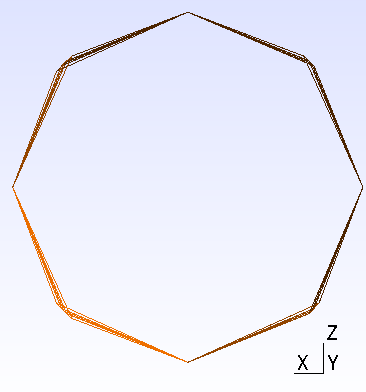
\includegraphics[height=0.6\textheight]{wire-cross-section.png}

        \scriptsize Wire cross section.
      \end{center}
    \end{column}
    \begin{column}{0.5\textwidth}
      \begin{center}
        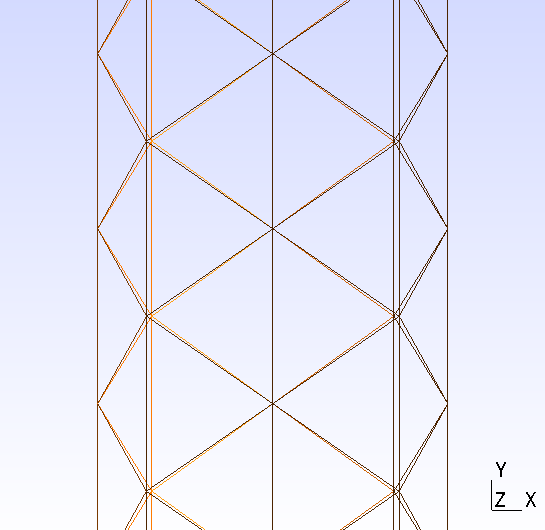
\includegraphics[height=0.6\textheight]{wire-side-section.png}

        \scriptsize Wire side view.
      \end{center}
    \end{column}
  \end{columns}
  
  \begin{itemize}
  \item Trade-off between mesh granularity and CPU time.
  \end{itemize}
\end{frame}

\begin{frame}
  \frametitle{An Initial E-Field Calculation}
  \begin{columns}
    \begin{column}{0.5\textwidth}
      \begin{center}
        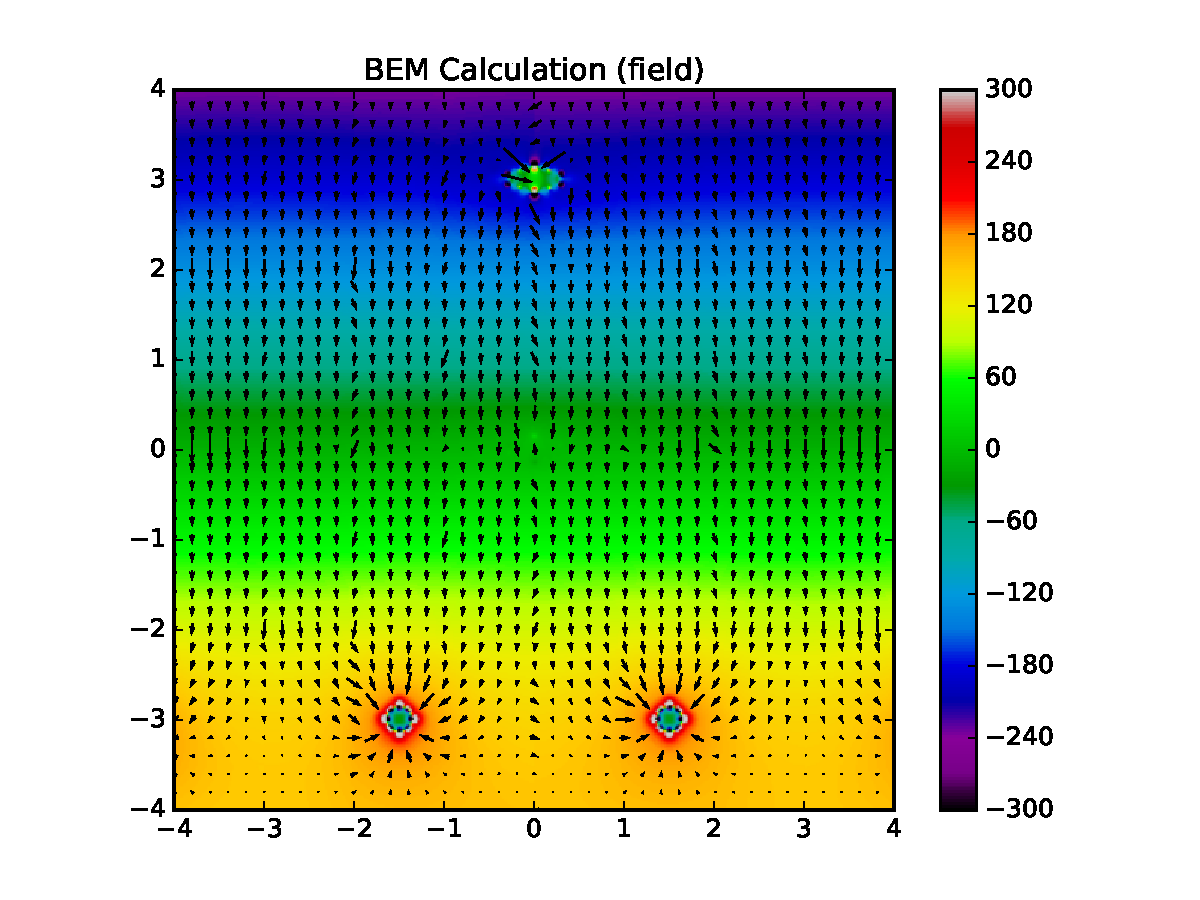
\includegraphics[height=0.6\textheight]{uboone-drift-field-pot-tight.pdf}

        \scriptsize E-field lines on top of potential.
      \end{center}
    \end{column}
    \begin{column}{0.5\textwidth}
      \begin{center}
        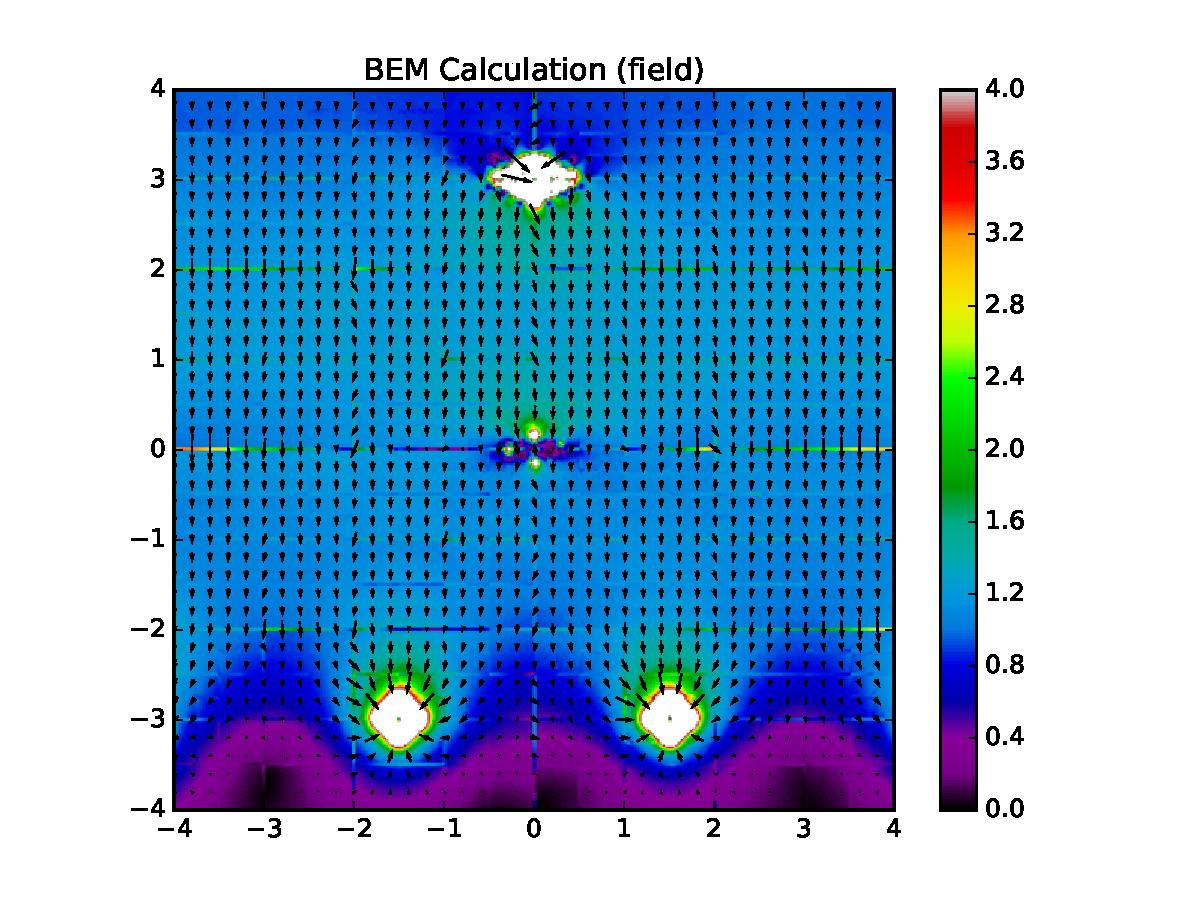
\includegraphics[height=0.6\textheight]{uboone-drift-field-tight.pdf}

        \scriptsize E-field lines on top of $\left|\vec{E}\right|$.
      \end{center}
    \end{column}
  \end{columns}
  
  \begin{itemize}
  \item Trade-off between mesh granularity and CPU time.
  \end{itemize}
\end{frame}


\section{Software}

\begin{frame}{Status of Field Calculations}
  \tableofcontents[currentsection]
\end{frame}

\begin{frame}
  \frametitle{Main Dependencies}

  \href{http://www.bempp.org/}{BEM++}
  \begin{itemize}
  \item Solves Laplace, Helmholtz and Maxwell eqns using BEM
  \item C++ with Python interface.
  \item General, but low-level.  Requires some understanding.
  \item Multithreaded.
  \end{itemize}

  \href{http://gmsh.info}{GMSH}
  \begin{itemize}
  \item 3D Grid generator and visualization.
  \item Volume and surface meshes.
  \item Interactive and scripted geometry definition.
  \end{itemize}

  Python:
  \begin{itemize}
  \item NumPy, Matplotlib and \textbf{LARF}
  \end{itemize}
\end{frame}

\begin{frame}[fragile]
  \frametitle{LARF - Liquid ARgon TPC Field Calculator}

  \footnotesize

  For now, code lives at:
  \begin{center}
    \url{https://github.com/brettviren/larf}
  \end{center}

\begin{verbatim}
$ larf mesh -o uboone.msh ubone
$ gmsh uboone.msh     # <-- to visualize the generated mesh
$ larf solve -d 11 -g near -o uboone-near-d11.npz uboone.msh
$ larf plot -p near -o uboone-near-d11.pdf uboone-near-d11.npz
\end{verbatim}

  Processing directed by a \texttt{larf.cfg} configuration file, specify things like:
  \begin{description}
  \item[geometry] naming the mesh generators and parameters
  \item[problem] to \text{solve} (weighting vs drift)
  \item[gridding] to use for both the solution and and any plots
  \item[plot] describing what plotting code to apply to a solution
  \end{description}

  \begin{itemize}
  \item Solution results are saved as Python NumPy array files.
  \item Will extend this as the to-do list is tackled.
  \end{itemize}



\end{frame}

\section{To do}

\begin{frame}{Status of Field Calculations}
  \tableofcontents[currentsection]
\end{frame}

\begin{frame}
  \frametitle{Much Still To Do}

  \begin{itemize}
  \item Include calculations for DUNE detector geometry.
  \item Visualize E-fields, do more careful comparisons to 2D
    results.
  \item Go from 2D slices to full 3D volumetric data.
  \item Dynamics:
    \begin{itemize}\footnotesize
    \item Charge drifting and wire-current signal generation.
    \item Let's make a new simulated animation!
    \end{itemize}
  \item Responses as a function of position.
    \begin{itemize}\footnotesize
    \item Repeat Yichen's study on intra- and inter-wire-regions
    \end{itemize}
  \item Finally, develop some response functions for signal extraction.  
    \begin{itemize}\footnotesize
    \item How detailed? (per-plane?, per wire?)
    \item How to validate?
    \end{itemize}
  \item Other ideas:
    \begin{itemize}\footnotesize
    \item Jim: Edge effects near field cage, TPC-TPC gaps, inside APA.
    \item Milind: calculate transparency of induction planes.
    \item Others?
    \end{itemize}
  \end{itemize}

\end{frame}

\begin{frame}
  \frametitle{Other Efforts - FEM}
  \begin{columns}
    \begin{column}{0.5\textwidth}
      \footnotesize

      Leon Rochester @ SLAC
      \begin{itemize}\scriptsize
      \item \href{http://microboone-docdb.fnal.gov:8080/cgi-bin/ShowDocument?docid=5892}{\microboone DocDB 5892}
      \item FEM using custom code (``DIY Garfield'')
      \item C++ rewritten from ICARUS FORTRAN.
      \item Good looking initial results on drift field and with particle stepping.
      \item I expect we will do a systematic comparison at some point.
      \end{itemize}
      Manhong Zhao @ BNL
      \begin{itemize}\scriptsize
      \item Initial discussions to do FEM using ANSYS + the ``multi physics'' module.
      \item Beefy workstation on order.
      \end{itemize}
      \vspace{3mm}
      \textbf{Not to forget hardware-based measurements!}
    \end{column}
    \begin{column}{0.5\textwidth}
      \begin{center}
        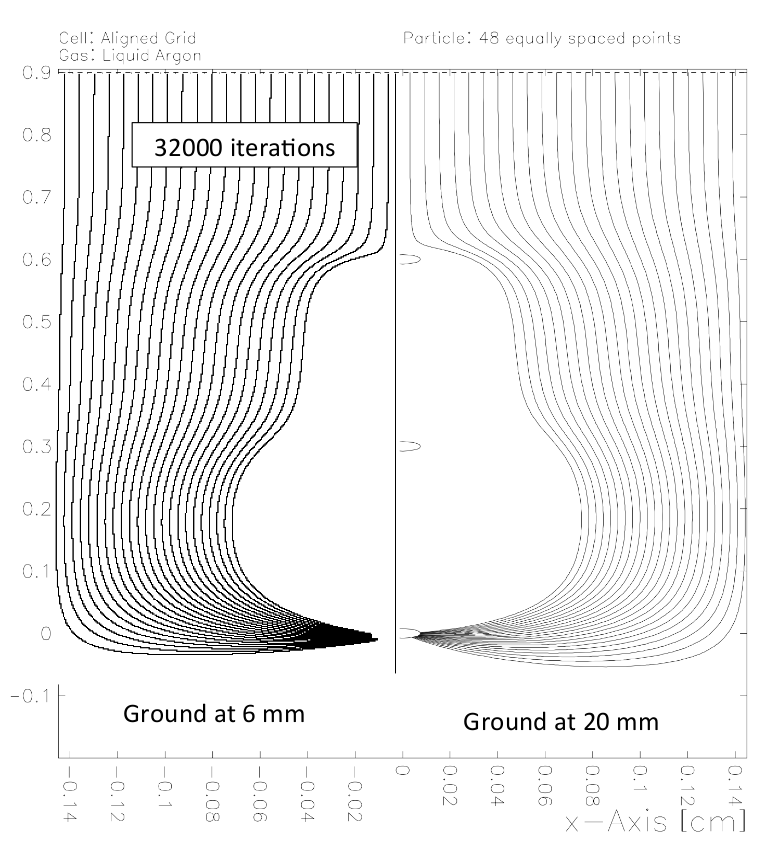
\includegraphics[width=\textwidth]{leon-32kiter.png}

        \scriptsize Left half is Leon's FEM after 32k iterations with Garfield 2D on right half.
      \end{center}

    \end{column}
  \end{columns}

  

\end{frame}


\end{document}
